\documentclass[]{beamer}
\usepackage{tikz,lstautogobble,listings}
\usetikzlibrary{arrows.meta}
\usetheme{Rochester}
\usepackage[T1]{fontenc}
\usepackage[utf8]{inputenc}
\lstset{
  language=caml,
  basicstyle=\ttfamily\tiny,
  breaklines=true,
  autogobble=true,
}


\title{TIPE 25/26 - Cycles et Boucles}
\author{GIL Dorian}
\subtitle{Méthode des tableaux : Optimisation pour les clauses de Horn}
\date{}

\begin{document}

\begin{frame}
\titlepage
\end{frame}

\begin{frame}{Sommaire}
\begin{enumerate}
    \item Présentation Méthode
    \item Exemple d'Application
    \item Implémentation en OCaml
    \item Objectifs futurs
\end{enumerate}
\end{frame}

\begin{frame}{Présentation}
    \begin{definition}[Méthode des tableaux]
        Algorithme pour prouver une assertion $\phi$ ayant pour hypothèse $(H_n)$ en montrant
        que $\lnot \phi$ est insatisfaisable.
    \end{definition}
    \begin{definition}[Clause de Horn]
        Clause (i.e con/disjonction de littéraux) comportant au plus un littéral positif
    \end{definition}
    \pause
    \begin{itemize}
        \item On place $\lnot\phi$ et ses hypothèses dans la racine.
        \item On applique des règles $(R_x)$ à chaque formule en bout d'arbre qui sont developpables
        \item Si on trouve $a$ et $\lnot a$ dans l'arbre (un \textit{cycle}), alors $\phi$ est vrai
    \end{itemize}
    \pause
    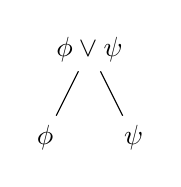
\begin{tikzpicture}[scale=0.75]
    \node {$\phi\lor\psi$}
        child {node {$\phi$}}
        child {node {$\psi$}};
    \end{tikzpicture}
    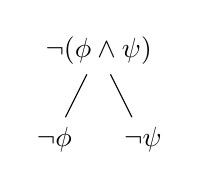
\begin{tikzpicture}[scale=0.75]
    \node {$\lnot(\phi\land\psi)$}
        child {node {$\lnot\phi$}}
        child {node {$\lnot\psi$}};
    \end{tikzpicture}
    \begin{tikzpicture}[scale=0.75]
    \node {$\lnot\lnot\phi$}
        child {node {$\phi$}};
    \end{tikzpicture}
    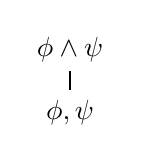
\begin{tikzpicture}[level distance=8mm]
    \node {$\phi\land\psi$}
        child {node {$\phi, \psi$}};
    \end{tikzpicture}  
    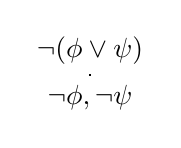
\begin{tikzpicture}[level distance=8mm,scale=0.75]
    \node {$\lnot(\phi\lor\psi)$}
        child {node {$\lnot\phi, \lnot\psi$}};
   \end{tikzpicture}
    Les règles
\end{frame}


\begin{frame}{Exemple}
    \textbf{Formule:} $a \Rightarrow (b \Rightarrow a)$

    \begin{center}
        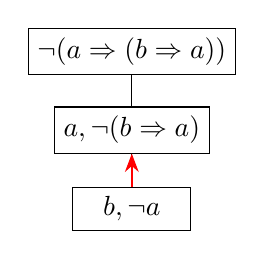
\begin{tikzpicture}[
            every node/.style={draw, minimum width=1.5cm, align=center},
            every arrow/.style={thick,->,>=Stealth}
        ]
        \node (root) at (0,0) {$\lnot(a \Rightarrow (b \Rightarrow a))$};
        \pause
        \node (not_b_a) at (0,-1) {$a, \lnot(b \Rightarrow a)$};
        \draw[thin] (root) -- (not_b_a);
        \pause
        \node (b) at (0,-2) {$b, \lnot a$};
        \draw[thin] (not_b_a) -- (b);
        \pause
        \draw[red, every arrow, thick] (b) -- (not_b_a);
        \end{tikzpicture}
    \end{center}
\end{frame}

\begin{frame}[fragile]{Implémentation 1}
    \begin{center}
        \begin{tabular}{c}
            \begin{lstlisting}
                type formula =
                    | Atom of string
                    | Not of formula
                    | And of formula * formula
                    | Or of formula * formula

                let rec expand formula =
                    match formula with
                    | Not (Not f) -> [[f]]
                    | Not (And (f1, f2)) -> [[Not f1]; [Not f2]]
                    | Not (Or (f1, f2)) -> [[Not f1; Not f2]]
                    | And (f1, f2) -> [[f1; f2]]
                    | Or (f1, f2) -> [[f1]; [f2]]
                    | _ -> [];;

                let rec has_cycle branch =
                    List.exists (fun f -> List.mem (Not f) branch) branch;;
            \end{lstlisting}
        \end{tabular}

    Première implémentation en OCaml, sans les hypothèses
      \end{center}
\end{frame}

\begin{frame}[fragile]{Implémentation 2}
    \begin{center}
        \begin{tabular}{c}
            \begin{lstlisting}
                let rec tableau branches =
                    match branches with
                    | [] -> false
                    | branch :: rest -> 

                    if has_cycle branch then
                        tableau rest
                    else
                        match branch with
                        | [] -> true
                        | f :: fs ->

                        let expansions = expand f in match expansions with
                        | [] -> tableau (fs :: rest)
                        | new_branches ->
                        
                        let expanded_branches = List.map (fun b -> b @ fs) new_branches in
                        tableau (expanded_branches @ rest);;

                    let is_satisfiable formula =
                    let initial_branch = [formula] in tableau [initial_branch];;
            \end{lstlisting}
        \end{tabular}

    Première implémentation en OCaml, sans les hypothèses
      \end{center}
\end{frame}

\begin{frame}{Ce qui est à faire}
    Mon but sur le long terme
    \begin{itemize}[<+->]
        \item Ajouter les hypothèses à l'implémentation et faire les preuves de correction, terminaison pour toutes formules.
        \item Trouver et prouver des optimisations.
        \item Implémenter et commenter les résultats de l'optimisation.
        \item Faire de même en logique du première ordre OU continuer à trouver des optimisations dans la logique propositionelle.
    \end{itemize}
    \pause
    Sur le court terme :
    \begin{itemize}[<+->]
        \item Ajouter les hypothèses à l'implémentation.
        \item Faire les preuves de correction, terminaison pour toutes formules.
        \item Commencer la recherche d'optimisation
    \end{itemize}
\end{frame}
\end{document}